\section{LSST Observing Cadence Optimization to Enhance PHA Completeness \label{sec:opsim}}

The effects of varying the LSST observing strategy on PHA completeness and other science can be evaluated in detail
using a combination of the LSST Operations Simulator (OpSim) and the LSST Metrics Analysis Framework (MAF).
The LSST Metrics Analysis Framework (MAF) is a user-oriented, python package for evaluating the pointing history
from these simulated surveys in light of particular science goals or interests. The various metrics coded in the
MAF framework can be calculated for any given simulated survey and compared as proposal parameters are changed
in OpSim. This permits a thorough investigation of the trades between different observing strategies, in terms of the
effect on science goals, including the PHA completeness.  We first describe the basic steps in our simulations,
then describe the baseline and modified LSST simulated surveys, and then discuss our results.


\subsection{Simulations of LSST Asteroid Discoveries}

The basic components of our end-to-end simulation of asteroid discovery, described in detail below, include
\begin{enumerate}
\item {\it NEO Population Modeling.} Orbital parameters are used to generate asteroid positions during the
simulated survey duration for a simulated or properly debiased extant NEO population. The population needs
to adequately sample color, size and other properties. A database of such positions evaluated with an adequate
time step  is available as an input to MAF.
\item {\it Survey Cadence Modeling.} A series of LSST pointings with instrumental metadata and observing conditions
is generated by OpSim. In addition to boresight positions, the camera orientation and selected filter, available
metadata enable the computation of instrumental sensitivity (limiting magnitudes).
\item {\it Asteroid Optical Flux Modeling.}  Optical flux from an arbitrary asteroid needs to be computed
as a function of the positions of the Sun, the asteroid and Earth, and asteroid physical properties (e.g., size
and color). This model is implemented in MAF.
\item {\it Source Detection Modeling.} Given the instrument model, observing conditions and asteroid flux,
the signal-to-noise ratio is estimated and used to compute detection probability. This model is implemented
in MAF.
\item {\it Detection Linking Modeling.}  Instead of running MOPS, a model that emulates MOPS
performance is used to significantly speed up the computations. This model is implemented
in MAF.
\item {\it Completeness Estimation.} Given a list of ``discovered objects'', and the input population,
the completeness is estimated as a function of asteroid properties (e.g. size) and various other parameters
(e.g. observing strategy). This model is implemented in MAF.
\end{enumerate}

We proceed to describe these models in more detail, and then discuss the baseline and several modified LSST
surveys, and the corresponding PHA completeness estimates.

\subsubsection{NEO Population Modeling \label{sec:MAFdetails}}

We have chosen to use an orbital distribution defined by the large ($>1$ km) diameter known PHAs, as reported to the Minor Planet Center (MPC). This population is thought to be relatively complete and thus should be relatively unbiased. For comparison with other completeness estimates, we also evaluate completeness using a random sample of 2000 NEOs from the synthetic solar system model presented in \cite{Grav2011}.  A plot of the $a$, $e$, $i$ distributions for these PHAs and NEOs is shown in Figure~\ref{fig:PHA_orbits}.

For populations where the $H$ magnitude distribution is strongly correlated with their orbital distribution,
it is necessary to specify an $H$ magnitude (needed for incoming flux computation) for each object. However, most small body populations, including the PHA population larger than 140~m in diameter, can be well described by independent orbital and $H$ magnitude distributions. In this case, a smaller set of orbits can be used to represent the overall larger population; during analysis, each object can be `cloned' from the fiducial $H$ magnitude associated with the orbit to a range of $H$ magnitudes covering the range interesting for analysis (corresponding to a shift of apparent $m_V$ magnitude). This makes the metric analysis, and particularly the generation of the expected observations for each object, simpler and faster. As long as sufficient resolution of the orbital parameter space is maintained, the metric results over the range of $H$ magnitudes will be comparable to the results calculated with a larger population. Here we use the small population of $>1$~km diameter known PHAs and NEOs, then clone them to a range of $H$ magnitudes between $H$=11 and $H$=28 using $dN/dH = 10^{\alpha\, H}$, with $\alpha$ = 0.3. We have verified with a larger, simulated set of NEOs that reducing the population from 10,000 model NEOs to 2,000 model NEOs does not change the calculated survey  completeness.

Using the details of the input population, MAF then generates the expected observations of each object using the pointing history
from a specific OpSim simulated survey. Ephemerides are generated using OpenOrb \citep{OpenOrb2009} for a closely spaced grid
of times (typically every 2 hours), and then interpolated to the exact times of each OpSim pointing.


\begin{figure}[t!]
\centering
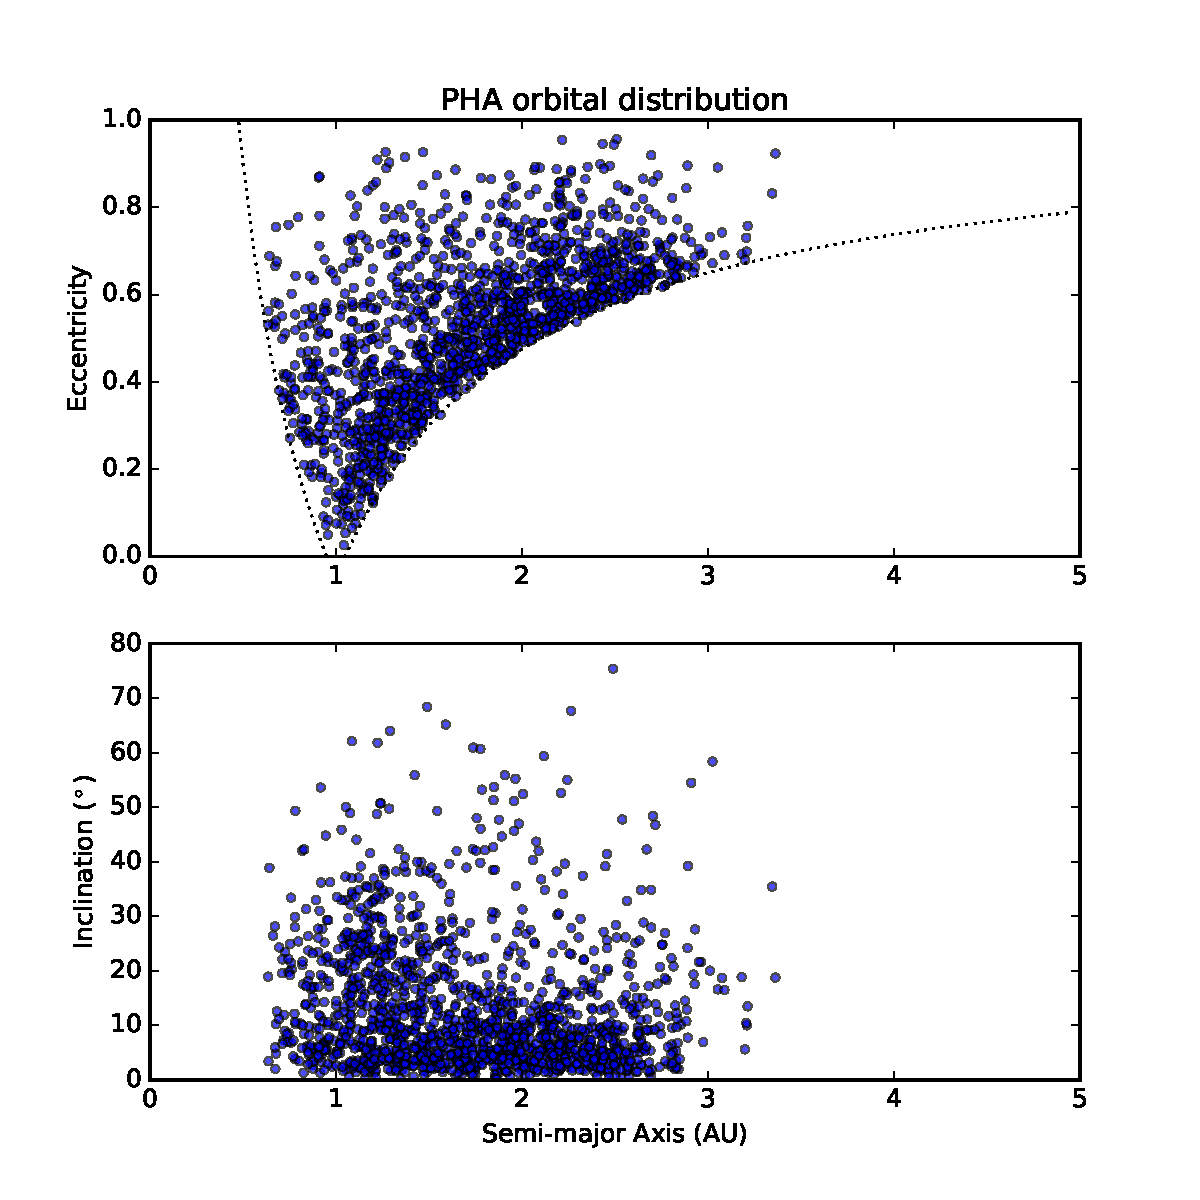
\includegraphics[width=0.49\textwidth]{figures/pha20141031_orbits}
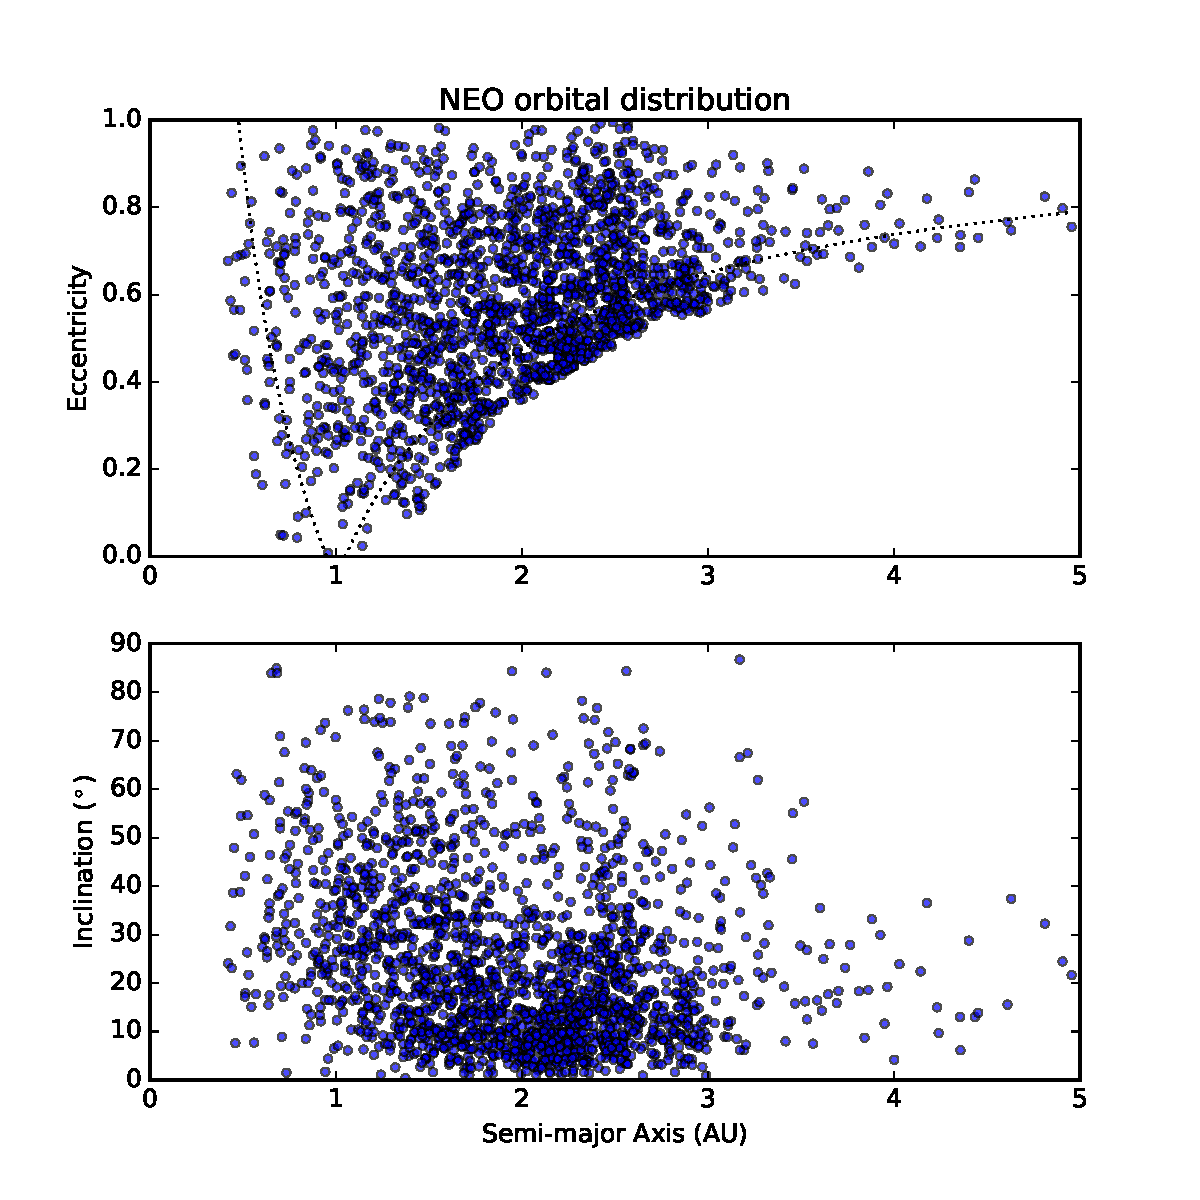
\includegraphics[width=0.49\textwidth]{figures/neos_2k_orbits}
\vskip -0.2in
\caption{The eccentricity and inclination distributions, as a function of semi-major axis, of the PHAs (left) and NEOs (right) used in this analysis. The PHA population consists of the orbital distribution of $>1$~km PHAs recorded by the MPC as of 2014 (1511 objects). The NEO population is a random sampling of 2000 NEOs from the S3M \citep{Grav2011}, a synthetic solar system model based on the \cite{Bottke2002} NEO orbital distribution. NEOs are defined as objects with $q<1.3$~AU; PHAs are defined as having a Minimum Orbit Intersection Distance (MOID) with the Earth of less than 0.05~AU (implying $q\le1.05$~AU) and having $H\le22$.  \label{fig:PHA_orbits}}
\end{figure}

\subsubsection{Survey Cadence Modeling}

The LSST Operations Simulation \citep[OpSim,][]{delgado14} is a python software package that generates a realistic pointing history, with the time, filter, location, astronomical conditions, weather conditions, and predicted point-source $5\sigma$ limiting magnitude, for each LSST visit
for, typically, ten years. This pointing history is generated using weather data (cloudiness and seeing) from the Cerro Pachon site and a high-fidelity model of the telescope itself (including slew and settle time and dome movement, for example), combined with a parameterized set of observing proposals that determine how the scheduling algorithm attempts to gather observations. By configuring OpSim with different parameters for the observing proposals, we can generate a series of simulated surveys which prioritize different science goals. The LSST baseline survey and its modifications designed to enhance the PHA completeness are described in detail
in \S\ref{sec:surveys} below.


\subsubsection{Asteroid Optical Flux Modeling}

Given $H$ magnitude for an object, its apparent magnitude in Johnson's $V$ band can be easily computed
given the positions of the object, the Sun and the observer (e.g. \citealt{juric02}).
Magnitudes, or fluxes, in any other optical and near-IR band (in case of LSST, $u$, $g$, $r$, $i$, $z$, and $y$)
can be computed from $V$ magnitude by specifying a spectrum or relevant colors for each object. We have
assumed that our entire PHA population has the same colors as C-type main-belt asteroids, with resulting
transformations to  LSST bandpasses listed in Table~\ref{tab:sed_colors}. Choosing the colors of  S-type
main-belt asteroids instead results in $<$1\% changes in completeness.

\begin{deluxetable}{ccccccc}
\centering
\tablecolumns{7}
\tablecaption{Color transformations from Johnson's $V$ band to LSST bandpasses, for C and S type asteroids. \label{tab:sed_colors}}
\tablewidth{0.7\textwidth}
\tablehead{ Type & $V-u$ & $V-g$ & $V-r$ & $V-i$ & $V-z$ & $V-y$  \\ }
\startdata
C  & -1.53 &  -0.28 &  0.18 &  0.29 &  0.30 & 0.30 \\
S & -1.82 &  -0.37 &  0.26 & 0.46 &  0.40 & 0.41  \\
\enddata
\end{deluxetable}


\subsubsection{Source Detection Modeling}


\begin{figure}[t!]
\centering
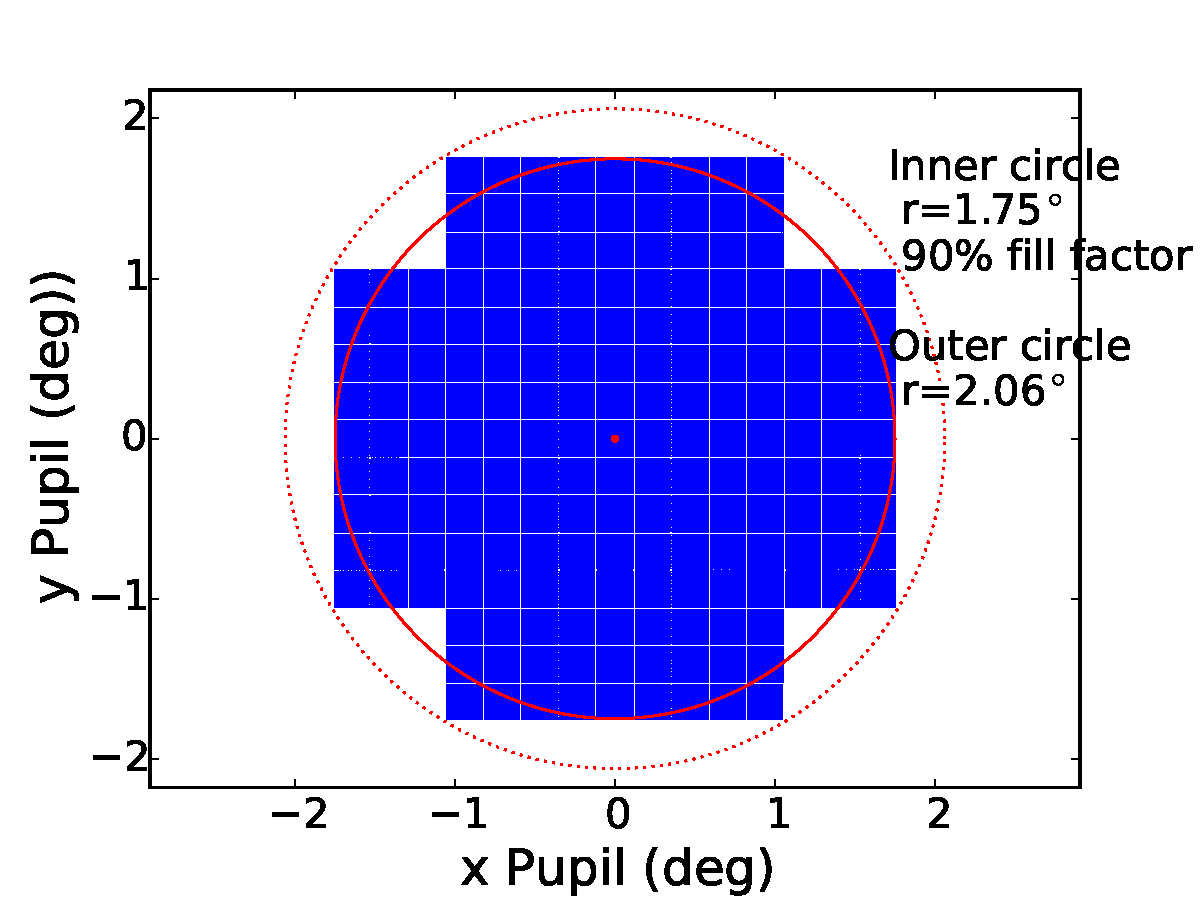
\includegraphics[width=0.65\textwidth]{figures/focalplane}
\caption{Model of the LSST camera footprint, including chipgaps and CCD + raft layout. \label{fig:camera_footprint}}
\end{figure}

If the object is within the LSST field of view, its predicted position, velocity, and apparent $V$ magnitude (calculated from the fiducial $H$ magnitude associated with the orbit) is recorded along with information about the simulated observation itself (such as the seeing, limiting magnitude, filter, and boresight RA/Dec). The full LSST camera footprint, including chipgaps, is used to determine whether
an object is within the field of view. The LSST camera footprint is shown in Figure~\ref{fig:camera_footprint}.

MAF also calculates trailing loss estimates for each observation, which are necessary when evaluating if a particular object is visible in a given observation. Trailing losses occur whenever the movement of an object spreads its photons over a wider area than a simple stellar point spread function (PSF). There are two aspects of trailing loss to consider: SNR losses and detection algorithm losses. The first is the
irreversible degradation in SNR that occurs because the trailed object includes a larger number of background pixels in its footprint, compared to a stationary PSF. The second effect, detection loss, occurs because source detection software is optimized for detecting point sources; a stellar PSF-like matched filter is used when identifying sources that pass above the defined threshhold. This filter is non-optimal for trailed objects but losses can be mitigated with improved software ({\it e.g.} detecting to a lower PSF-based SNR threshhold and then using a variety of trailed PSF filters to detect sources). When considering whether a source would be detected at a given SNR using typical source detection software, the sum of SNR trailing and detection losses should be used. With an improved
algorithm optimized for trailed sources (and this with additional workload on data management), the smaller SNR losses should be
used instead.

\begin{figure}[t!]
\centering
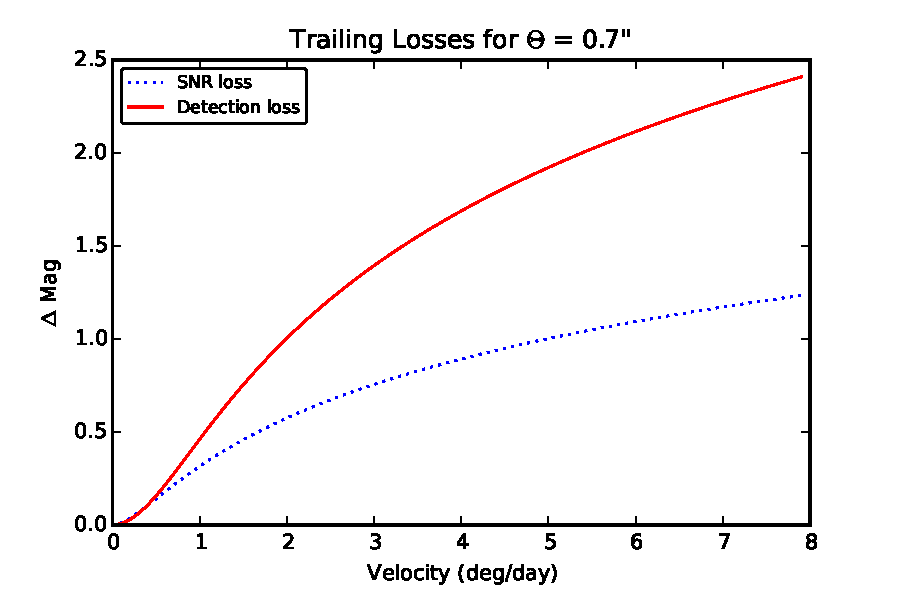
\includegraphics[width=0.85\textwidth]{figures/trailing_losses}
\caption{Trailing losses for 30 second LSST visits, assuming seeing of
  0.7''. The dotted line shows SNR trailing losses, the solid line
  indicates cumulative losses that also account for non-optimal detection
  algorithm. With software improvements the latter detection losses can be
  mitigated. At the fiducial $v=1$ deg/day, the SNR loss is $\sim$0.3 mag,
  and non-optimal detection algorithm contributes an additional loss of
  $\sim$0.16 mag.
\label{fig:trailinglosses}}
\end{figure}

Our simulations of these effects show that both trailing losses can be fit well with the
same functional form:
\begin{eqnarray}
\Delta \, m & = &-1.25 \, log_{10} \left( 1 + \frac{a \, x^2} { 1 + b\,
    x} \right) \\
x & = & \frac{v \, T_{exp}} {24 \, \theta}
\end{eqnarray}
where $v$ is the velocity (in deg/day), $T_{exp}$ is the exposure time (in seconds), and $\theta$ is the FWHM (in arcseconds). For trailing SNR losses, we find $a = 0.67$ and $b = 1.16$; for the cumulative loss, that includes both SNR and detection losses,
we find $a=0.42$ and $b=0$. An illustration of the magnitude of these trailing loss effects for 0.7 arcsec seeing is given in Figure~\ref{fig:trailinglosses}.

We calculate the probability of detecting a particular source given its magnitude $m$ (after accounting for trailing losses)
and the $5\sigma$ limiting magnitude $m_5$ using a logistic function
\begin{eqnarray}
     P & = & \left[ 1 +  {\rm exp}\left(\frac {m -  m_5}{\sigma}\right) \right]^{-1}.
\end{eqnarray}
where $\sigma$=0.12 describes the width of the completeness falloff \citep{2014ApJ...794..120A}. A source is randomly classified
as detected using the probability $P$. We also evaluate more optimistic discovery criteria using only SNR trailing losses
(i.e. without taking detection losses into account), as well as detections to SNR=4 instead of SNR=5.


\subsubsection{Detection Linking Modeling}

Given the set of visits where the object was within the field of view and detected, we look for visits spaced in time
according to the discovery criteria. These criteria generally consist of a given number of visits within a specified
time span within a single night, followed by a given number of additional nights (each with the same required number
of visits in the same time span) falling within a specified time window. The basic criteria is a pair of visits in each
night occurring within 60 minutes, repeated for 3 nights within a 15 day time window. However, we also evaluate
the effect of varying the discovery criteria to require triplets or quads of visits within a single night, and increase
the length of the search window from 15 to 30 days.


\subsubsection{Completeness Estimation}

With each unique set of discovery criteria, we have a record of what objects would be ``discovered'' at each $H$ value.
With this we calculate the differential discovery completeness, the fraction of objects discovered at a given $H$ magnitude.
To turn this into a cumulative discovery completeness, we simply integrate over $H$, assuming a given $H$ distribution
for the population (recall that we use $dN/dH = 10^{\alpha\, H}$, with $\alpha$ = 0.3).


\subsection{OpSim Simulated Surveys \label{sec:surveys}}

\subsubsection{The LSST Baseline Survey}

The current baseline observing strategy for LSST is represented by our reference run, minion\_1016. This simulated survey
contains observations balanced between several different observing proposals:
\begin{enumerate}
\item The Wide, Fast, Deep (WFD) proposal (also known as the Universal proposal) is the primary LSST survey, expected to receive about 90\% of the observing time and to cover 18,000 deg$^2$ of sky. In the baseline observing strategy, this proposal is configured to obtain visits in pairs spaced about 30 minutes apart, and will typically return to each field about every 3-4 days, balancing the six $ugrizy$ filters. The footprint for the WFD proposal covers approximately $+5^\circ$ to $-60^\circ$ in declination, with a full range of RA values except for a region around the Galactic plane. This declination range corresponds to an airmass limit of about 1.3 when the fields are at an Hour Angle of $\pm$2 hours. In minion\_1016, the WFD proposal receives 85\% (2,083,758) of the total number of visits.
\item The North Ecliptic Spur (NES) proposal is an extension to the WFD to reach the northern limits of the Ecliptic plane ($+$10 degrees), and allows higher airmass observations. The visit timing is similar to the WFD, although the $u$ and $y$ filter are not requested in this region. In the baseline observing strategy, minion\_1016, each NES field requests about 40\% of the total number of WFD visits per field when considering $griz$ filters only (304 visits per field in $griz$ vs 795 visits per field in $griz$ in WFD), and receives 6\% (158,912) of the total number of visits.
\item The Deep Drilling Fields (DD) proposal includes a set of single pointings that are requested in extended sequences; currently these sequences are $grizy$ visits, with additional coverage in $u$ band. Each sequence requires about an hour of observing time, and is repeated every few days. In minion\_1016, there are 5 DD fields, 4 of which correspond to fields which have been officially selected
by the Project and announced to the community; these five fields receive 5\% of the total visits.
\item The Galactic Plane (GP) proposal covers the region with high stellar density around the Galactic plane not covered by the WFD. This proposal requests a small number of visits in each of the six $ugrizy$ filters, with no timing constraints. In minion\_1016, this proposal receives 2\% of the total visits.
\item The South Celestial Pole (SCP) proposal is an extension of the WFD footprint to cover the region south of $-60^\circ$ declination. Like the GP, this proposal requests a small number of visits in each of the six $ugrizy$ filters, with no timing constraints. In minion\_1016, this proposal receives 2\% of the total visits.
\end{enumerate}

The footprint of these various proposals in the baseline minion\_1016 reference run is shown in Figure~\ref{fig:minion_footprints}. In each proposal, the individual visits are 30 seconds long, consisting of two back-to-back coadded 15 second exposures.

\begin{figure}[t!]
\centering
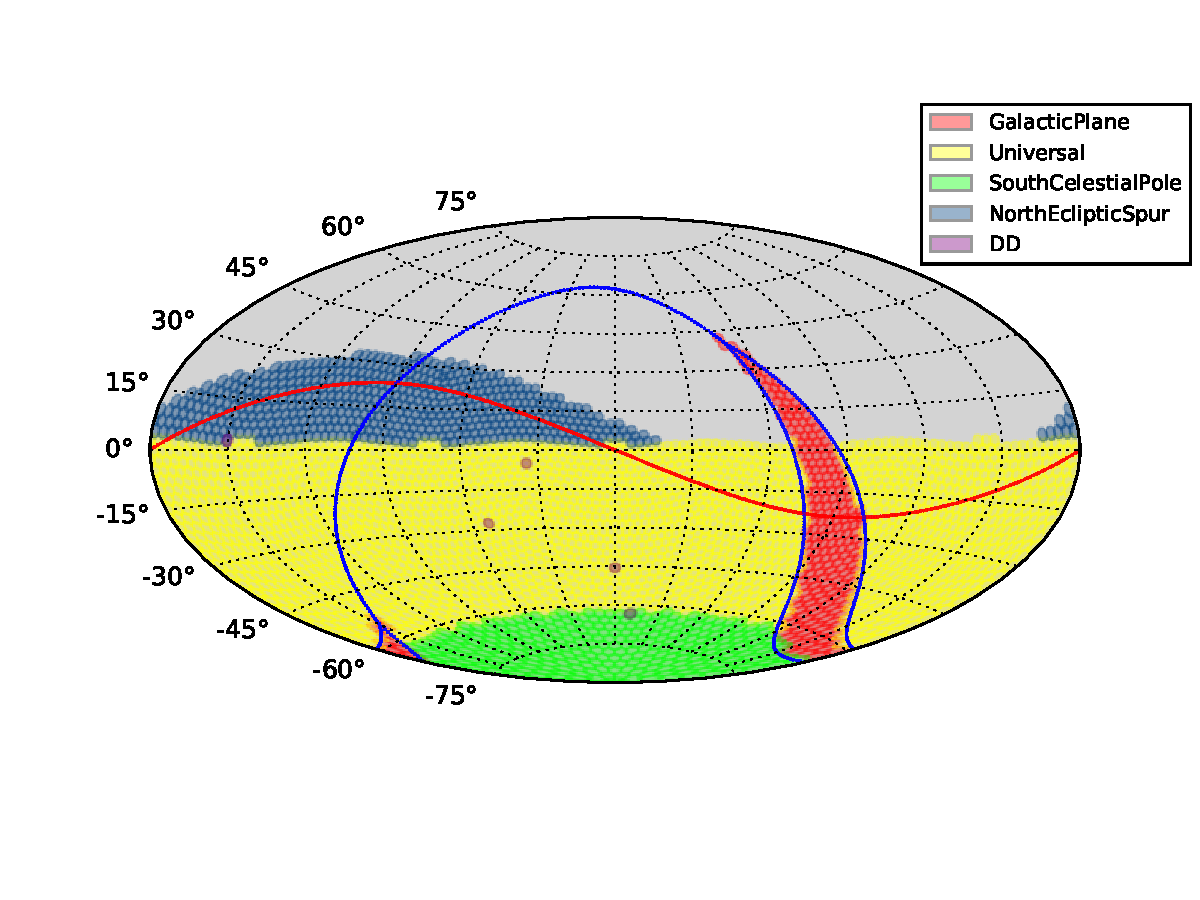
\includegraphics[width=0.85\textwidth]{figures/minion_1016_proposal_footprint}
\vskip -1.0in
\caption{The footprints of the various proposals included in the baseline observing strategy, represented by reference run minion\_1016.
\label{fig:minion_footprints}}
\end{figure}


\subsubsection{Modified Surveys}

A series of additional OpSim simulated surveys were created with parameters intended to improve the efficiency of discovering PHAs and increase the cumulative PHA completeness. They span the range from minor modifications to extreme changes that would
jeopardize other LSST science goals. We consider the latter in order to assess what would be ultimate performance of an
LSST-like system fully dedicated to NEO surveying.

\textbf{Extra ecliptic spur visits:} The first cadence change is simply to increase the number of visits requested for the NES proposal in $griz$, to increase the likelihood of discovering objects near the northern portion of the Ecliptic plane, and to extend the survey from 10 years to 15 years, increasing the discovery rate of PHAs with long synodic periods. Other proposals remain the same as in minion\_1016. Reprioritizing the NES relative to the WFD results in the WFD receiving 69\% (2,561,334 visits over 15 years) of the total visits and the NES receiving 24\%, compared to 85\% and 6\% respectively in the baseline strategy. The resulting simulated survey is astro\_lsst\_01\_1016.  We consider astro\_lsst\_01\_1016 as our 'baseline PHA' run, as it makes minimal changes to the overall survey strategy while attempting to be more PHA friendly.

\textbf{Longer ecliptic visits:} This simulation introduce an Ecliptic Band (EB) proposal, requesting observations with visit timing similar to the WFD in the $griz$ filters, but with field locations surrounding the Ecliptic Plane $\pm15^\circ$ and extending down to the WFD where the Ecliptic reaches its northernmost  range. This proposal replaces the NES proposal, and requests longer 60 second visits in order to reach deeper limiting magnitudes. Other proposals remain the same as in astro\_lsst\_01\_1016. With this reprioritization, the WFD receives 44\% (1,159,319) of the total visits while the EB receives 53\%; the simulated survey is astro\_lsst\_01\_1015.

\textbf{NEO-focused survey:} An attempt at an aggressively NEO-optimized survey was also created, where modified versions of the EB and WFD proposals are used. The visit timing in each proposal is the same as the standard WFD visit timing (a pair of visits separated by about 30 minutes), however the WFD footprint is changed to simply cover the entire area between 0$^\circ$ and $-60^\circ$ declination except for the EB footprint. The EB and WFD proposals request observations in only $gri$ filters, with 30 second visits in the WFD and 60 second visits in the EB. No other proposals are included. The resulting simulated survey is astro\_lsst\_01\_1017.

\begin{figure}[t!]
\centering
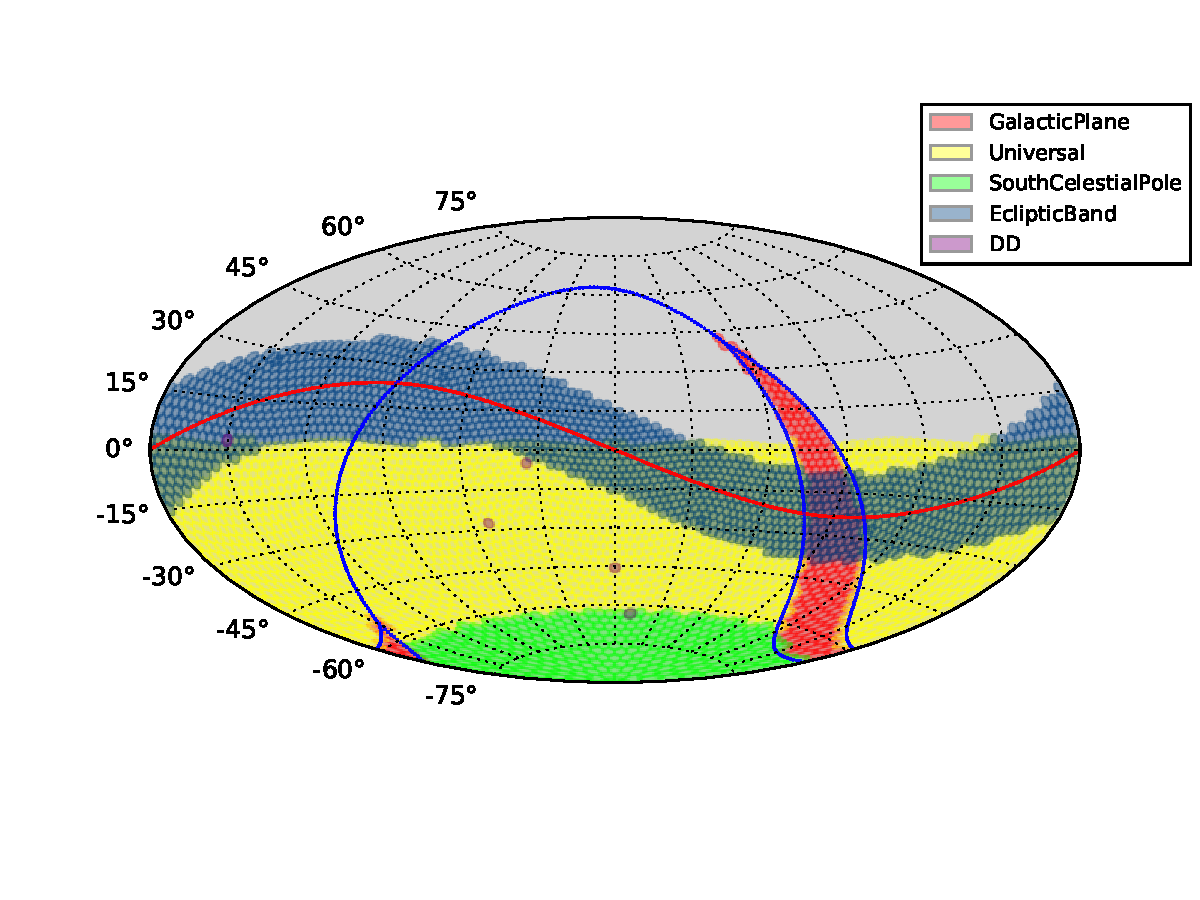
\includegraphics[width=0.49\textwidth]{figures/astro_lsst_01_1015_proposal_footprint}
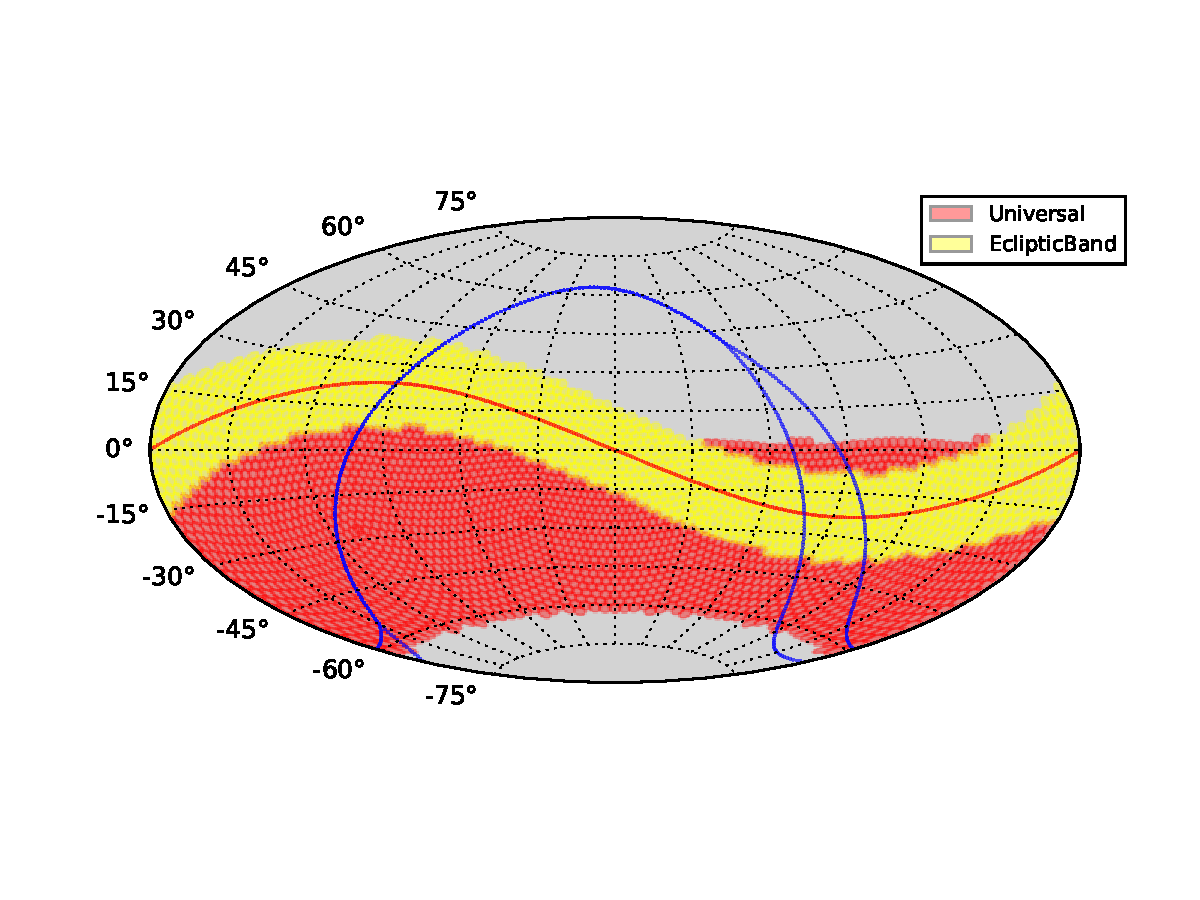
\includegraphics[width=0.49\textwidth]{figures/astro_lsst_01_1017_proposal_footprint}
\vskip -0.5in
\caption{The footprints of the proposals, including the Ecliptic Band proposal, used in the NEO-optimized simulated surveys astro\_lsst\_01\_1015 (the ``extra ecliptic visits'' survey, left) and astro\_lsst\_01\_1017 (the ``NEO-focused'' survey, right). The astro\_lsst\_01\_1017 survey only includes two proposals.
\label{fig:neo_footprints}}
\end{figure}


\subsection{Completeness analysis results}

In the baseline reference run, minion\_1016, with the baseline discovery
criteria, with pairs of visits in each night occurring within 60 minutes
repeated for 3 nights within a 15 day time window, we find a cumulative
completeness at $H\le22$ of 73.7\% for our PHA input population (see
Figure~\ref{fig:minionC1}). This should be considered our baseline PHA
completeness, as it uses the reference run and the baseline MOPS and data
management requirements.

From this baseline, we can evaluate the effects of changing both the survey design (reallocating telescope resources) and the discovery criteria, which effectively sets the computational resources.
There is an interplay between discovery criteria and survey design -- as an obvious example, discovery criteria requiring triplets of visits per night instead of pairs will result in much different completeness results if the survey was designed to only request two visits per night rather than three. Likewise, some changes in survey design work best with changes to the discovery criteria; for example, lengthening the visit time increases the detection losses, which means pushing source detection to the ``trailing loss'' threshold results in a significant improvement in completeness. While we compare discovery criteria within a single simulated survey as much as possible, there are some changes in discovery criteria which must be compared between different surveys using different observing strategies.

All the completeness results presented below assume that no objects are known prior to LSST survey,
and thus are biased low. For example, assuming that 43\% objects would be discovered by the start of
LSST survey, \cite{GMS2016} boosted the final PHA completeness for LSST baseline survey by as much
as 11\%.


\begin{figure}[t!]
\centering
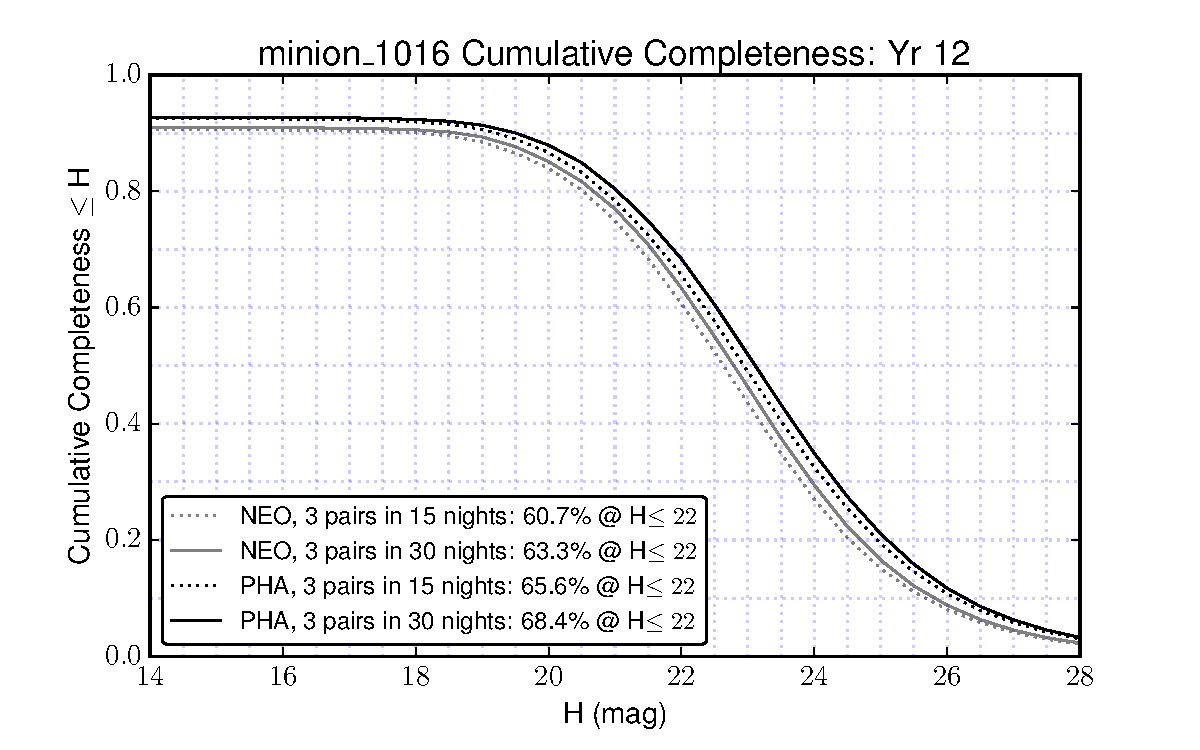
\includegraphics[width=0.99\textwidth]{figures/minion_1016_CumulativeCompleteness_NEO_and_PHA_Cumulative_Completeness}
\vskip -0.2in
\caption{The cumulative completeness for PHAs and NEOs, as a function of absolute magnitude $H$, for the baseline
cadence minion\_1016. \label{fig:minionC1}}
\end{figure}

\begin{deluxetable}{lccccccc}
\tablecaption{The cumulative completeness for PHAs with $H\le22$ for various
survey strategies (rows) and discovery criteria (columns). In addition to
changing the overall duration of the survey (12 years instead of 10), the
completeness is shown for different track linking windows (W=15 or 30 days),
enhanced detection algorithms to reduce trailing losses (``Trail Det''), and
pushing the individual detection threshold from SNR$=5$ to SNR$=4$. These are
primarily computational changes, while the various rows show different survey
cadences. These range from the current baseline, to adding additional visits or
longer visits in the ecliptic region, to focusing the majority of the time on
performing a NEO-focused survey. \label{tab:completeness}}
\tablehead{
& \multicolumn{3}{c}{10 year survey}  &  \multicolumn{4}{c}{12 year survey}  \\
\cmidrule(r){2-4} \cmidrule(r){5-8}
Simulation  & W=15 & W=30 & W=30 & W=15 & W=30 & W=30 & W=30 \\
            &      &      & Trail Det&  & & Trail Det & Trail Det \\
            &      &      &      &      & &           & SNR=4
}
\startdata
LSST baseline & 73.7 & 76.0 & 76.5 & & &  \\
Extra ecliptic visits & 74.8 & 76.8 & 77.4 & 79.1 & 80.8 & 81.5 & 83.8\\
Longer ecliptic visits & 73.6 & 77.4 & 79.5 & 77.5 & 80.9 & 82.9 & 85.6 \\
NEO-focused cadence & 76.2 & 79.0 & 80.6 & 79.9 & 82.5 & 83.9 & 86.0 \\
\enddata
\end{deluxetable}


\subsubsection{Modified Discovery Criteria \& Computational Strategies}

% Below, we explore the effects of changing the MOPS requirements, changing data management detection requirements, and changing the survey strategy.

Using only the baseline minion\_1016 and not changing the survey strategy, we can explore the impact on PHA completeness of changing the discovery criteria. These are correspond primarily to the different columns of Table~\ref{tab:completeness}, and include:

\begin{itemize}
\item extending the MOPS window for linking pairs of detections from the nominal 15 day window to a 30 day window: this increases completeness by about 2\%, although with an estimated increase in the compute requirements by about an order of magnitude (see Appendix \ref{sec:appMOPS}).
\item enhancing source detection algorithms to mitigate detection losses to the trailing loss level: with the 30 second visits in the baseline minion\_1016, this only increases completeness by a very small amount, 0.5\%.
\item using sources detected down to SNR=4 instead of SNR=5: this increases completeness by about 2\%, although with an estimated increase in the compute requirements by about two orders of magnitude (see \S\ref{sec:kaiser}).
\end{itemize}

The major gain available in the baseline survey (or any survey with a maximum visit time of 30 seconds) is through increasing the MOPS linking window from 15 to 30 days. This allows more opportunities to capture the PHAs in a set of observations which meet the discovery criteria. It is worthwhile to note that the current OpSim behavior does not prioritize capturing large chunks of contiguous sky, and often leaves gaps in coverage from night to night. This behavior is likely related to the increase in completeness going from 15 day windows to 30 day windows; with the large LSST field of view, after 30 days the areal coverage will be much more evenly distributed than after 15 days. Changes to the scheduling algorithm to favor covering contiguous blocks of sky\footnote{A similar modification of
the baseline cadence, the so-called ``rolling cadence'', is also favored by the supernovae science programs. A release of a series of simulated surveys implementing this idea is anticipated for late 2017.} are likely to improve the completeness even further.  Pushing to SNR=4 exceeds the expected compute resources and is not worthwhile in comparison.


When an NEO population is used instead of a PHA input population, the cumulative completeness is between 10-15\% lower
(see Figure~\ref{fig:minionC1}). This is primarily due to differences in their orbital distributions, as illustrated in Figure~\ref{fig:PHA_orbits}. The definition of PHAs includes a Minimum Orbit Intersection Distance (MOID) with Earth of 0.05~AU, requiring PHAs to more closely approach Earth than NEOs (which are defined as simply having $q<1.3$~AU), and thus the PHAs achieve brighter peak V magnitudes than the NEOs. To quantify this effect, we calculated the apparent $V$ magnitude for both the NEO and PHA input populations every night for ten years, while accounting for trailing losses and assuming a constant $H=22$ magnitude for every member of the population. The resulting distributions of the
brightest 10-year $V$ magnitude are shifted by about a magnitude (the mean values are 23.44 for NEOs and 22.42 for PHAs).


\subsubsection{The Performance of Modified Surveys}

The potential improvement in PHA discovery rates for modified survey cadences is
summarized in the rows of Table~\ref{tab:completeness} and described below.

\begin{itemize}
\item \textbf{Extra ecliptic spur visits:} By adding these extra visits over the course of a 10 year survey, the increase in completeness over the LSST baseline is about 1\%. This improvement comes at a cost to other science cases, as the main survey footprint (the WFD proposal) only receives 1,715,354 visits (82\%) of the number of visits in the reference run; the outcome of many science programs is roughly proportional to the number of visits.
\item \textbf{Extending the survey by two years:} Since minion\_1016 is a reference run, it only simulates 10 years.
However, we can evaluate the ``extra ecliptic visits'' run at the 12 year mark, at which point the WFD proposal has received approximately the same number of visits as it would receive in the baseline 10 year survey. The additional two years of operations adds just over 4\% to the completeness, going from 74.8\% at 10 years to 79.1\% at 12 years.
\item \textbf{Longer visits in the ecliptic:} This reaches fainter limiting magnitudes, but the effect of longer exposures alone is minimized by the fact that detection losses are also increased. It is also hard to disentangle the effects of increasing the visit time near the Ecliptic and the resulting lower frequency of observations (and thus fewer opportunities for sets of observations matching the basic discovery criteria). The small modifications made by this survey strategy show almost no change in completeness, {\it until} detection losses are partially compensated for by modifying source detection algorithms to the trailing loss level; then this run provides a 1.5\% increase in completeness compared to the ``extra ecliptic visits'' survey.
\item \textbf{Aggressively NEO-focused survey:} This survey uses a limited filter set, discards other proposals, and uses longer exposures along the ecliptic. This survey shows an increase in completeness (83.9\%), relative to the ``extra ecliptic visits'' survey of about 2.4\%, after using longer MOPS windows and pushing source detection to the trailing loss level.
However, many science programs would be jeopardized with this observing strategy because observations in the $uzy$ filters,
and observations of the DD and SCP fields, would not be obtained.
\end{itemize}

To summarize, when altering the survey strategy the largest individual gain ($\sim$5\%)
comes from simply extending the survey lifetime from 10 to 12 years. For the case of PHAs and 30-day wide MOPS window,
the completeness can be boosted from 76\% after 10 years with minion\_1016 survey to 81\% after 12 years with
``extra ecliptic visits'' survey (recall that this completeness estimates do not account for the contribution of known objects).

\subsection{Systematic Effects due to Varying Modeling Assumptions \label{sec:syseff}}

As indicated by the above discussion, a number of systematic effects must be taken into account when
comparing different simulations of the same survey, as well as simulations of different surveys and observing
systems. It is unlikely that a meaningful quantitative comparison can be pushed beyond a level of a few percent
in completeness (in practice, the completeness of a given operating survey is best estimated using the object
re-discovery rate). Based on our analysis, the leading systematic effects in simulated completeness estimates are:
\begin{enumerate}
\item NEO vs. PHA difference. The completeness is about $\sim$10-15\% higher for PHAs than for NEOs;
for minion\_1016, the cumulative completeness is 73.4\% for PHAs and  60.8\% for NEOs.
\item Orbital parameter distribution for the simulated asteroid population (e.g. the Bottke model
             vs. the Granvik model); varying populations contribute completeness uncertainty of about a few percent)
\item Different sample definitions: $H<22$ vs. $D>140$m (as shown by \citealt{GMS2016}, completeness
           increases by $\sim$5\% when $H$-based criterion is used)
\item Variations of the ``discovery window'' (e.g., X visit pairs in N nights: changing N from 15 to 30 with X=3 increases
          completeness by about 3\%; changing X from 3 to 4 with N=15 decreases completeness by 6\%).
\item Uncertainties when predicting effective image depth (system throughput, variation of the detection efficiency
          with the signal-to-noise ratio, treatment of trailing losses); for a survey that has a completeness above 60\%,
          each additional {\it 0.1 magnitude of depth for a given survey cadence increases the completeness by another 1\%}.
\item Uncertainties when predicting asteroid's apparent flux (albedo distribution, phase effects, photometric variability
          due to non-spherical shapes, color distributions); assuming an uncertainty of 0.2 mag in the effective
          limiting magnitude, the corresponding  systematic uncertainty in completeness is about 2\%.)
\item Variations of the nominal detection threshold (if the detection threshold is changed from the
          signal-to-noise ratio of 5 or greater to 4 or greater, the completeness is boosted by 2-3\%;
          the difference between the optimal detection using trailed profile and point-spread-function
          detection, which is negligible for LSST baseline exposure time of 30 seconds, would be worth 2\%
          in completeness for doubled exposure time).
\item Sensitivity to details in sky coverage and cadence (e.g. nightly pairs of visits vs. quads of visits;
          requiring quads instead of pairs of visits decreases completeness by 30\% using baseline cadence;
          about half of that loss can be recovered using cadence simulations that request four visits per night)
\item The slope of the asteroid size distribution (current measurement uncertainty of this parameter
          corresponds to a systematic uncertainty in completeness of about 2\%.)
\item The impact of known objects: assuming that 43\% objects would be discovered by the start of
          LSST survey, \cite{GMS2016} boosted the final PHA completeness for LSST baseline survey by 11\%.
\end{enumerate}

We proceed with an example of a comparison of different simulations.


\subsection{A Comparison with the Grav, Mainzer \& Spahr (2016) Study \label{sec:GMS}}

\cite[hereafter GMS]{GMS2016} reported different NEO completeness levels than published by the LSST team
in 2007 and 2014. Given the above discussion of various systematic effects, it is easy to understand
the reported differences. There are three main reasons why the GMS results differ:
\begin{enumerate}
\item GMS used a different realization of the LSST baseline survey.
\item GMS used different synthetic NEO populations to evaluate completeness.
\item GMS {\it redefined} the completeness limit from the commonly
  used $H<22$ criterion to an albedo-dependent value of $H$ limit (which
  attempts to directly model the $D>140$ m size cut).
\end{enumerate}

Regarding the last point, GMS found that the completeness drops by 5\% when $H<22$ criterion is
replaced by $D>140$ m criterion. Regarding  the first point, GMS results can be directly compared to an
LSST study by \cite{JJI2016}, who used the same simulated cadence. After accounting for the $H<22$ vs.
$D>140$ m methodological difference of 5\%, GMS obtained a completeness of 67\% when requiring
3 pairs of visits in 12 nights (for simulated cadence {\it enigma\_1189}), while the \citet{JJI2016}
study obtained $\sim$73\% using 3 pairs of visits in 15 nights (for simulated cadence {\it minion\_1016},
which is statistically very similar to {\it enigma\_1189}). This difference of $\sim$5\% is attributable to
the differences in simulated NEO populations and other modeling details. In summary, GMS find the NEO
completeness in the range $\sim$60\% to $\sim$70\% for the LSST baseline cadence. The range of values
is due to different NEO populations, varying NEO detection criteria, and other specifics. When accounting
for different choices of simulation parameters, the GMS results are fully consistent (within 1-2 \%) with
the results previously published by the LSST team, and with the results discussed here.
